\section{Causal Graph}

Given an event structure $\es = (E, \#, \vdash)$, we start by constructing
the lattice of \textbf{valid} configurations for $\es$. We then apply the following
transformations to this lattice:

For each edge $X \rightarrow X' = X \cup \set{e}$ in the graph,
where $X, X' \subseteq E$ and $e \in E$,
we add a new vertex $r_{X,X'}$, remove the edge $X \rightarrow X'$,
and introduce two new edges $X \rightarrow r_{X,X'}$, $r_{X,X'} \rightarrow X'$.

For each $S, e$ such that $S \vdash e$, we add a new vertex
(labelled as $m_{S,e}$) to the graph. For any pair of vertices
$X, X'$ in the graph, where $r_{X,X'}$ is also in the graph, we add
an edge from $m_{S,e}$ to $r_{X,X'}$ iff $S \subseteq X$ and
$\set{e} = X' \setminus X$. For consistency we re-label the configuration vertices
such that a given vertex $X$ is re-labelled as $x_{X}$.

Informally, the $r$- and $m$-vertices are added to show the
induction steps, as defined in Prop. \ref{prop:es-induction},
for constructing the initial lattice.

\begin{exmp}\label{ex:es}
Consider the event structure $\es = (E, \#, \vdash)$,
where:
\begin{equation*}
\begin{split}
  E      & = \set{a, b, c} \\
  \#     & = \varnothing \\
  \vdash & = \set{
    (\varnothing, a), (\set{a}, b), (\set{a}, c), (\set{b}, c)
  }
\end{split}
\end{equation*}

The causal graph for $\es$ is as depicted in Fig. \ref{fig:es-causal-graph}.

\begin{figure}
\centering
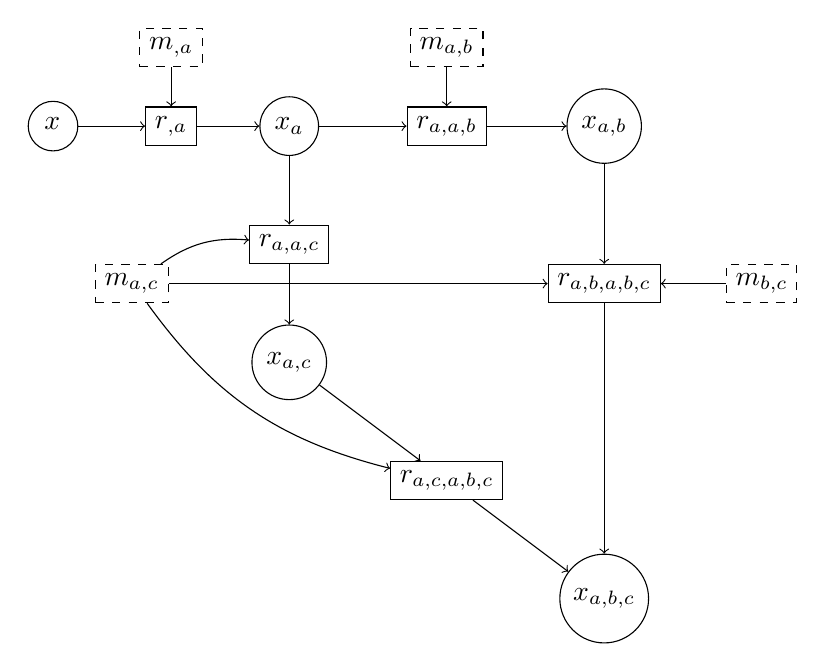
\begin{tikzpicture}
  \tikzset{
    _x/.style={circle,draw},
    r/.style={rectangle,draw},
    m/.style={rectangle,draw,dashed},
  };
  \node[_x] (_x-null) at (0,0)  {$x_{\varnothing}$};
  \node[_x] (_x-a)    at (3,0)  {$x_{\set{a}}$};
  \node[_x] (_x-ab)   at (7,0)  {$x_{\set{a,b}}$};
  \node[_x] (_x-ac)   at (3,-3) {$x_{\set{a,c}}$};
  \node[_x] (_x-abc)  at (7,-6) {$x_{\set{a,b,c}}$};

  \node[r] (r-null-a) at (1.5,0)  {$r_{\varnothing, \set{a}}$};
  \node[r] (r-a-ac)   at (3,-1.5) {$r_{\set{a}, \set{a,c}}$};
  \node[r] (r-a-ab)   at (5,0)    {$r_{\set{a}, \set{a,b}}$};
  \node[r] (r-ab-abc) at (7,-2)   {$r_{\set{a,b}, \set{a,b,c}}$};
  \node[r] (r-ac-abc) at (5,-4.5) {$r_{\set{a,c}, \set{a,b,c}}$};
  
  \node[m] (null-en-a) at (1.5, 1) {$m_{\varnothing, a}$};
  \node[m] (a-en-b)    at (5,1)    {$m_{\set{a}, b}$};
  \node[m] (a-en-c)    at (1,-2)   {$m_{\set{a}, c}$};
  \node[m] (b-en-c)    at (9,-2)   {$m_{\set{b}, c}$};

  \draw[->] (_x-null)      -- (r-null-a);
  \draw[->] (r-null-a)  -- (_x-a);
  \draw[->] (_x-a)         -- (r-a-ab);
  \draw[->] (r-a-ab)    -- (_x-ab);
  \draw[->] (_x-a)         -- (r-a-ac);
  \draw[->] (r-a-ac)    -- (_x-ac);
  \draw[->] (_x-ab)        -- (r-ab-abc);
  \draw[->] (r-ab-abc)  -- (_x-abc);
  \draw[->] (_x-ac)        -- (r-ac-abc);
  \draw[->] (r-ac-abc)  -- (_x-abc);
  \draw[->] (null-en-a) -- (r-null-a);
  \draw[->] (a-en-b)    -- (r-a-ab);
  \draw[->] (a-en-c)    -- (r-ab-abc);
  \draw[->] (b-en-c)    -- (r-ab-abc);
  \draw[->] (a-en-c) edge[bend left=20]  (r-a-ac);
  \draw[->] (a-en-c) edge[bend right=20] (r-ac-abc);
\end{tikzpicture}
\caption{Causal graph for Ex. \ref{ex:es}}
\label{fig:es-causal-graph}
\end{figure}

\end{exmp}

\begin{prop}
Given an event structure with $n$ events, constructing the
described causal graph requires $\mathcal{O}(2^n)$ operations.
\end{prop}